\section{Update phase}

The main computation in the update phase is {\tt valid}
cross-correlation between an image of forward propagation and an image
of backward propagation. We will refer to these as image and gradient,
respectively.  This cross-correlation could be done with an approach
similar to Algorithm \ref{alg:serial-forward-subtask} for forward and
backward propagation, which is the strategy suggested in
Refs. ~\cite{chellapilla2006high,das2016distributed}.  However, the
output of the update is an image with the same size as the kernel,
which is typically very small.  In this regime, the sub-image
primitive may not be efficient.  Therefore, we take a different
approach, defining the following stack of primitives:
  \begin{enumerate}
    \item {\bf Sub--kernel primitive} computes a cross--correlation of
      each of $S$ images of size $R_x \times R_y \times (Z + R_z - 1)$
      with $S$ gradients of size $1 \times 1 \times Z$ to produce and
      accumulate the results of $S^2$ kernel gradients of size $R_x
      \times R_y \times R_z$.  As in the propagation algorithm, this
      primitive is optimized for efficiently reusing the register file
      as well as $L1$ cache.
    \item {\bf Full kernel primitive} computes cross--correlation of
      an arbitrary sized $S$ images with arbitrary sized $S$ gradients
      to produce $S^2$ kernel gradients.  Optimized for hardware
      pre--fetching and efficient use of higher levels of cache.
    \item {\bf Sub--layer primitive} computes $\beta \times \beta'
      \times S^2$ kernel gradients by cross--correlating each of
      $\beta S$ images with $\beta' S$ gradients.
    \item {\bf Full layer primitive} divides the computation into a
      set of previous primitives and statically schedules execution.
      As described below, this primitive might need to contain an
      extra reduction step.
  \end{enumerate}


  \begin{algorithm}
    {\footnotesize
      \begin{codebox}
        \Procname{$\proc{Update-Subtask} \langle R_x, R_y, R_z, Z, R_s \rangle(i,\hat{i}',\Delta w)$}
        \li \kw{simd register} $oreg[R_x][R_y][R_z][R_s]$
        \li \kw{simd register} $wreg$
        \li \For $s_0 \gets 0 \To S/R_s - 1$
        \li \Do $oreg[:][:][:][s_0R_s:s_0R_s+R_s-1][:] \gets$
        \li   \Do $\proc{LOAD}(\Delta w[:][:][:][s_0R_s:s_0R_s+R_s-1][:])$
        \End
        \li \For $z_g \gets 0 \To Z-1$ \Comment Partially unrolled
        \li   \Do $wreg \gets \proc{LOAD}(\hat{i}'[1][1][z_g][:])$
        \li   \For $x \gets 0 \To R_x-1$ \Comment Fully unrolled
        \li   \Do \For $y \gets 0 \To R_y-1$  \Comment Fully unrolled
        \li   \Do \For $z \gets 0 \To R_z-1$  \Comment Fully unrolled
        \li   \Do \For $s_1 \gets 0 \To R_S-1$   \Comment Fully unrolled
        \li   \Do $oreg[x][y][z][s_0 \cdot R_s + s][:] \gets \proc{FMADD}($
        \li   \Do $wreg,$
        \li       $\proc{EXLOAD}(i[x][y][z+i][s_0 \cdot R_s + s]),$
        \li       $oreg[x][y][z][s_0 \cdot R_s + s][:])$
        \End
        \End \li \kw{end for} $s$
        \End \li \kw{end for} $x$
        \End \li \kw{end for} $y$
        \End \li \kw{end for} $z$
        \End \li \kw{end for} $i$
        \li $\Delta w[:][:][:][s_0R_s:s_0R_s+R_s-1][:] \gets$
        \li \Do $\proc{STORE}(oreg[:][:][:][s_0R_s:s_0R_s+R_s-1][:])$
        \End
        \End \li \kw{end for} $s_0$
      \end{codebox}
    \caption{Finest granularity update primitive.}
    \label{alg:serial-update-subtask}
    }
  \end{algorithm}

  {\bf Sub--kernel primitive} \quad The lowest level primitive is
  shown in Algorithm~\ref{alg:serial-update-subtask}.  Following the
  same principles as in the propagation sub--kernel primitive we
  vectorize the computation of $\Delta w[r_x][r_y][r_z][f][f']$ computed
  via {\small
  \[
  \sum_{z}
  i[r_x][r_y][r_z+z][f] \cdot \hat{i}'[r_x][r_y][r_z][f']
  \]
  } such that the values of $\Delta w[r_x][r_y][r_z][f][:]$ are computed
  via {\small
  \[
  \sum_{z}
  i[r_x][r_y][r_z+z][f] \cdot \hat{i}'[r_x][r_y][r_z][:]
  \]
  } Again, we recognize the reuse of $\hat{i}'[r_x][r_y][r_z][:]$ and
  re--order the loops appropriately.  In order to allow in--register
  computation, same constraints are imposed on $R_x \times R_y \times
  R_z \times R_s$ -- Maximal of $31$ for AVX512 and $10$ for SSE4, AVX
  and AVX2.  Additionally we allow only values for $R_s$ that divide
  $S$.  In order for the working set to fit inside the $L1$ cache, $Z$
  should be sufficiently small.  The number of bytes required for the
  working set equals $4S(R_xR_y+1)(R_z+Z-1)$.  For a given choice of
  $R_x, R_y$ and $R_z$, and given size of $L1$ cache, we
  conservatively choose $Z$ so that no more than half the cache is
  required for the working set.

  \begin{figure}
     \centering
     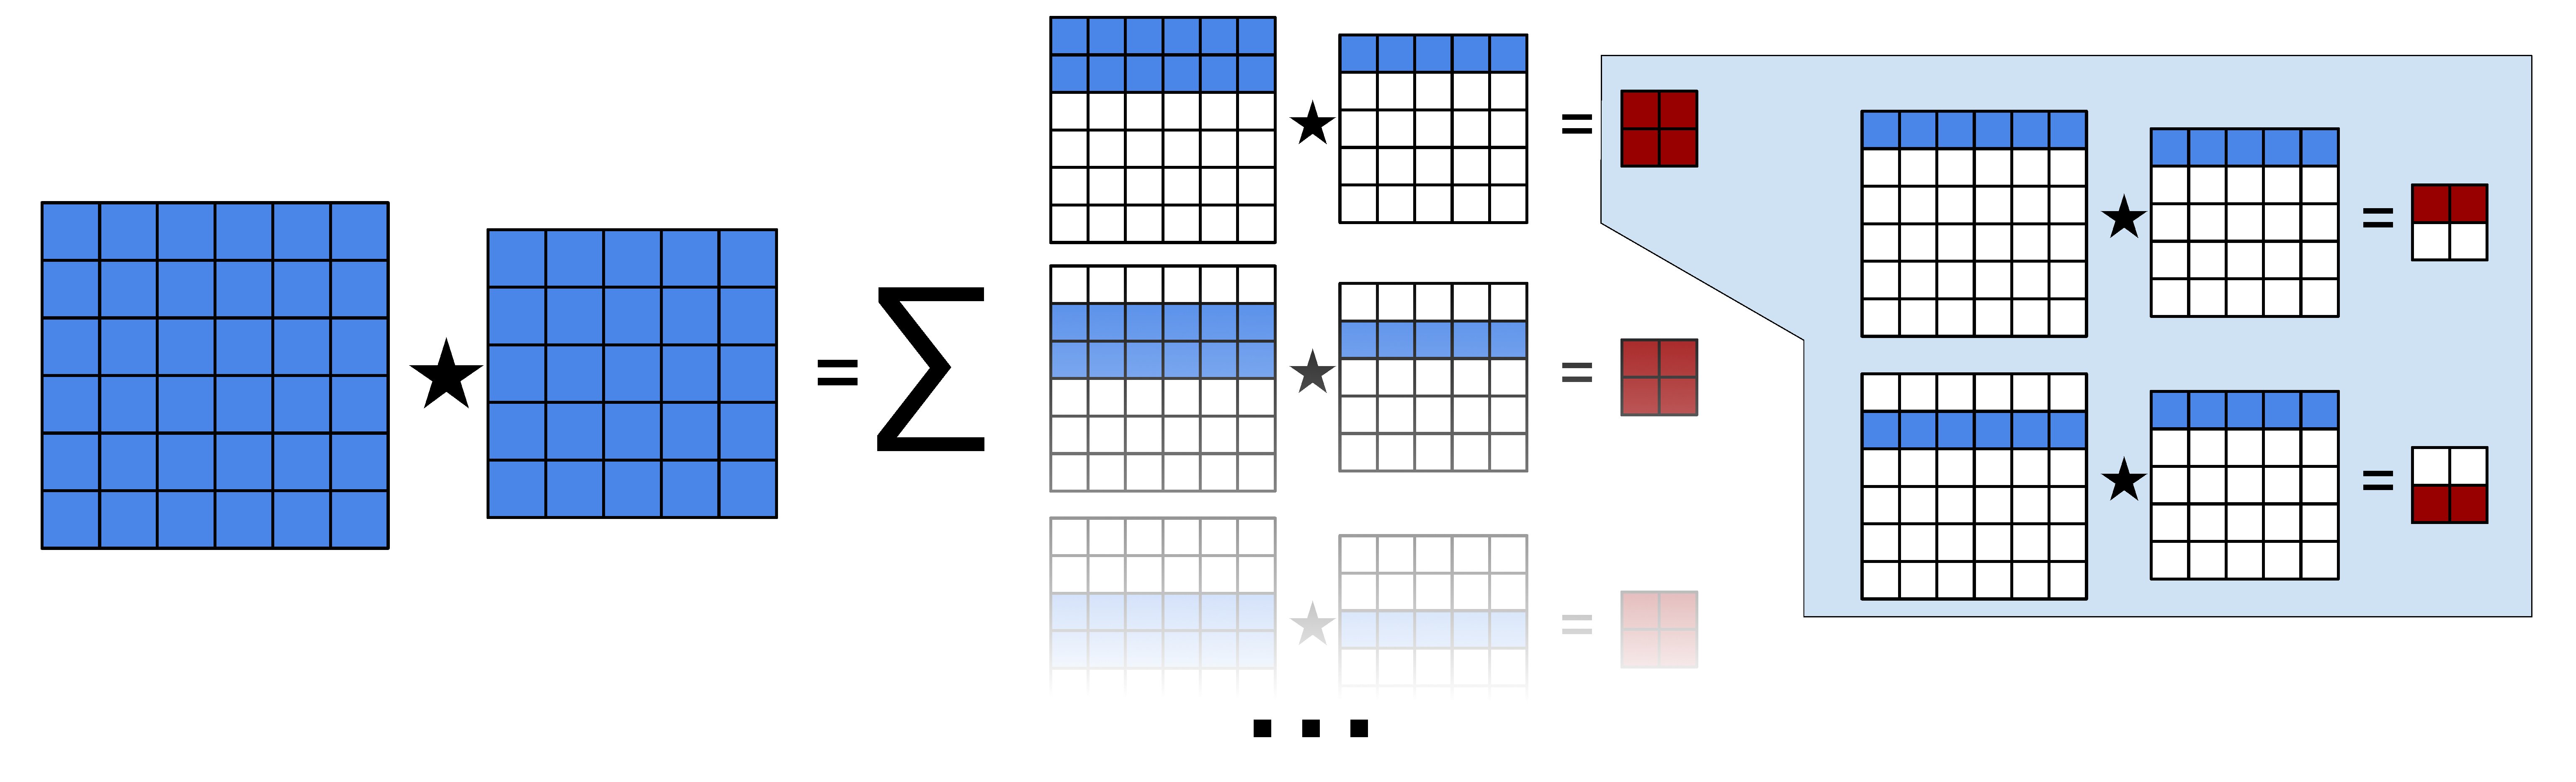
\includegraphics[width=0.99\linewidth]{fig/update2}
     \caption{An example of the {\bf full kernel primitive} and {\bf
         full gradient primitive} for the special case of $S=1$,
       $\vec{N}=\angled{1,6,6}$, $\vec{N}' = \angled{1,5,5}$ and
       $\vec{K}=\angled{1,2,2}$.}
     \label{fig:conv-decomposition}
   \end{figure}

  {\bf Full kernel primitive} computes $S^2$ kernel gradients by
  cross--correlating each of $S$ images with $S$ gradients.  The
  computation is performed in two steps.  First, the gradients are
  split into sub--gradients of size $1 \times 1 \times Z$.  The result
  is then obtained as the sum of cross--correlations of each of the
  sub--gradients with an appropriate sub--image, as depicted on
  Fig~\ref{fig:conv-decomposition} (middle column).  The
  cross--correlation of each sub--gradient is further split into
  sub--kernel primitives (right column on
  Fig.~\ref{fig:conv-decomposition}.  We choose the $R_x, R_y, R_z$
  and $R_s$ to maximize the register--file utilization, but subject to
  the limits described above.  Further, we require that $R_x, R_y$ and
  $R_z$ divide $K_x, K_y$ and $K_z$ respectively.  Note that this can
  always be accomplished by setting $R_x=R_y=R_z=1$ and $R_s=S$.
  However this choice might not be always optimal.  For example, when
  $K_z=3$ on AVX512 CPU, we could pick $R_s=8$ and $R_z=3$, as it
  utilizes $24$ registers, which is better than choosing $R_z=1$ and
  $R_s=S=16$.  The optimal division is the one for which $R_x \times
  R_y \times R_z \times R_s$ is maximized.  When more combinations are
  possible, we prefer ones with large values of $R_s$, then $R_z, R_y$
  and finally $R_x$.  The choice of $R_x, R_y, R_z$ and $R_s$ will
  determine the value of $Z$ as described above.  The computation is
  performed by iterating over $z$, then $y$, and then $x$.

  {\bf Sub--layer primitive} performs $\beta S \beta' S$
  cross--correlation.  Each of $\beta S$ input images is
  cross--correlated with each of $\beta'S$ output gradients to produce
  $\beta S \beta' S$ kernel gradients.  This primitive is designed for
  maximal reuse of higher levels of cache.  To achieve that, the
  computation is performed in the same fashion as in the propagation
  sub--layer primitive (Fig.~\ref{fig:full-exec}).

  {\bf Full layer primitive}, as in the propagation algorithm, divides
  the computation into sub--layer primitives which are scheduled for
  execution on $T$ threads.  In the propagation algorithm, all the
  divisions were done by splitting the relatively large output tensor,
  thus allowing each thread to perform an independent computation.  As
  our update sub--layer primitive always computes full kernel
  gradients, the only sub--division into independently computer
  results is possible along the two most significant dimensions of
  $\Delta W$ tensor (of sizes $F'$ and $F$).

  Further division can be accomplished by dividing the computation
  over the input images and output gradients.  A division can be
  performed across the batches $B$, such that separate threads
  consider only a subset of batches.  The resulting kernel gradients
  are then computed by accumulating the result obtained by each
  thread.  Similarly, a division can be performed by splitting the
  input image/output gradient as in the case of the {\bf full kernel
    primitive} (middle column of Fig.~\ref{fig:conv-decomposition}).

  To optimally divide the computation among threads we propose a two
  step scheduling algorithm.  In the first step, division along the
  two most significant dimensions of $\Delta W$ is performed to obtain
  independent sub--problems.  Let $P = \proc{GCD}(T,\alpha\alpha')$,
  we first select $\beta$ and $\beta'$ such that they divide $\alpha$
  and $\alpha'$ respectively, and $\beta\beta'P = T$.  Out of all
  possible values we pick the one for which $|\beta -\beta'|$ is
  minimized.  The threads are then also divided into $P$ sets of
  $T'=T/P$ threads, each of which will compute $\beta\beta'S^2$ kernel
  gradients.

  The values of the kernel gradient tensor $\Delta W(A
  \beta'S:A\beta'S+\beta'S-S,B \beta S: B\beta S + \beta S -S, :,:,:)$ is
  performed by the $A + B \alpha / \beta$-th set of $T'$ threads.

  In the second step, we divide the computation of each of
  $\beta\beta'S^2$ kernel gradients among the $T'$ threads in the set.
  When $T'$ equals $1$, the single thread in the set scheduled to
  perform the whole computation using a full layer primitive.

  When $T'>1$, we perform the division over input images and output
  gradients, creating a full layer primitive for each sub--problem.
  The division is performed in the same fashion as in the propagation
  algorithm, preferring divisions over $B$, then over $N_x'$, $N_y'$
  and finally $N_z'$.  However, each of the $T'$ threads in the set
  will accumulate the computed kernel gradients of each primitive into
  a local tensor.

  The $T'$ tensors computed by each thread have to be then accumulated
  to obtain the final kernel gradient tensor.  This is accomplished by
  performing a reduction step after all threads in the set have
  completed the execution.  The reduction requires little computation
  compared to the overall computation performed by the layer, and is
  thus performed by a single thread in the set.  During the reduction
  step both in--memory representations of the kernels are updated as
  well.
